\documentclass[xcolor=dvipsnames]{beamer}
%
% Choose how your presentation looks.
%
% For more themes, color themes and font themes, see:
% http://deic.uab.es/~iblanes/beamer_gallery/index_by_theme.html
%
\mode<presentation>
{
  \usetheme{Darmstadt}      % or try Darmstadt, Madrid, Warsaw, ...
  \usecolortheme{wolverine} % or try albatross, beaver, crane, ...
  \usefonttheme{structurebold}  % or try serif, structurebold, ...
  \setbeamertemplate{navigation symbols}{}
  \setbeamertemplate{caption}[numbered]
  % eigenen stuff definieren
    % auf dieser website stehen weiter elemente von denen die farbe geändert werden kann
    % http://www.cpt.univ-mrs.fr/~masson/latex/Beamer-appearance-cheat-sheet.pdf
    % einfach ausprobieren was passt
    \definecolor{Grau}{HTML}{CCCCCC}
    \definecolor{GrauDark}{HTML}{777777} % auf weißem hintergrund
    \definecolor{Orange}{HTML}{EA5B10}
    \setbeamercolor{palette primary}{bg=Grau}
    \setbeamercolor{palette primary}{fg=BurntOrange}
    \setbeamercolor{normal text}{fg=GrauDark}
    \setbeamercolor{structure}{fg=BurntOrange} % farbe der items
    \setbeamertemplate{itemize item}[circle]
    \setbeamercolor{mini frame}{fg=BurntOrange}
    \setbeamercolor{section in head/foot}{bg=Grau}
    \setbeamercolor{section in head/foot}{fg=BurntOrange}
    \setbeamercolor{subsection in head/foot}{bg=white}
    \setbeamercolor{subsection in head/foot}{fg=GrauDark}
    \setbeamercolor{headline}{bg=Grau}
    \setbeamercolor{block body}{bg=white}
    \setbeamercolor{frametitle}{bg=white}
    
} 

\usepackage[utf8]{inputenc}
\usepackage[T1]{fontenc}
\usepackage{ae}
\usepackage{ngerman}
\usepackage{calc}
\usepackage{graphicx}

\title[Team 2 - Implementierung]{CS:Select Implementierung - Team 2}
\author{Luca Springer, Alexander Linder, Julian Dinh, Nicholas Bieker,\\ Bendix Sonnenberg}
\date{06.02.2019}

\begin{document}

\begin{frame} % das ist eine slide
  \titlepage
\end{frame}

\section{Kriterien}

\begin{frame}{Muss-Kriterien}
  \begin{itemize}
    \item Verwalten des Systems durch Systemadministrator \\
    \item Anmeldemechanismus wurde umgesetzt (Registrierung, Login) \\
    \item Grafische Oberfläche von Java Server Pages dargestellt (Funktioniert in Chrome + Mozilla Firefox) \\
    \item Organisatoren: Spiele erstellen, Spieler spielen Spiel. Bewertung durch angebundenen ML-Server, Ergebnisse in Schema interner Datenbank gespeichert \\
    \item Die Modi MatrixSelect und BinarySelect wurden umgesetzt \\
    \item Punktesystem wurde umgesetzt \\
  \end{itemize}
\end{frame}

\begin{frame}{Kann-Kriterien (1)}
  \begin{itemize}
    \item Verwalten des Spiel-Servers möglich. Spiele aus Datenbank löschen und Server z.B über Docker herunterfahren - wichtige Daten zur Laufzeit in interner Datenbank gespeichert \\
    \item Erweiterte Nutzerverwaltung: Das Passwort soll in Zukunft zurücksetzbar sein, bis jetzt wurde das nicht implementiert \\
    \item Organisator: Löschen terminierter Spiele aus Übersicht, nicht terminierte Spiele frühzeitig beenden \\
    \item Streaks wurden eingeführt \\
    \item Spieler können Runden überspringen, es werden keine Punkte abgezogen - allerdings Streak abgebrochen \\
  \end{itemize}
\end{frame}
\begin{frame}{Kann-Kriterien (2)}
  \begin{itemize}
    \item Spieler können in einer Runde Merkmale als unwichtig markieren \\
    \item Es wurden keine weiteren Spielmodi hinzugefügt, Erweiterbarkeit im Großen aber beachtet \\
    \item Leaderboard, Achievements, Daily-Challenges wurden umgesetzt \\
    \item Hilfstexte \\
    \item Verbesserung der Merkmalsbereitstellung \\
    \item Internationalisierung (en/de) \\
    \item Unterstützung von mehreren Plattformen \\
  \end{itemize}
\end{frame}
\section{Schicke Implementierung}
\begin{frame}{Spieldarstellung}
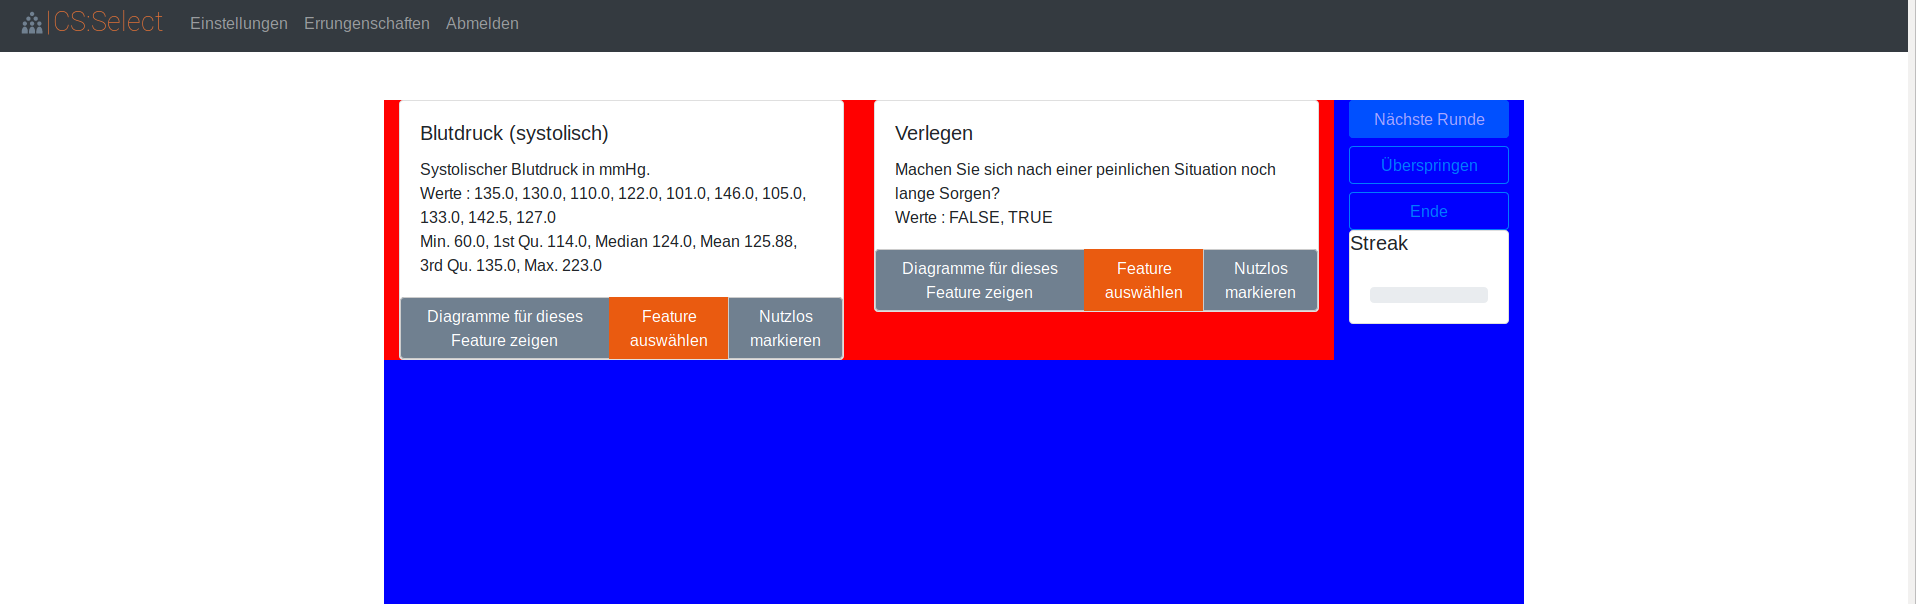
\includegraphics[width=\textwidth]{../img/gameframe.png}
\begin{itemize}
    \item Laden der Features passiert im Gameframe
    \item Aus der Rückgabe der API wird das Spiel gerendert
    \item Wenn das Spiel fertig ist wird ein Event ausgelöst, was den Next Button freischaltet
\end{itemize}
\end{frame}

\section{Zeitlicher Ablauf und Probleme}
\begin{frame}{Zeitlicher Ablauf und Probleme}
\begin{figure}
\centering
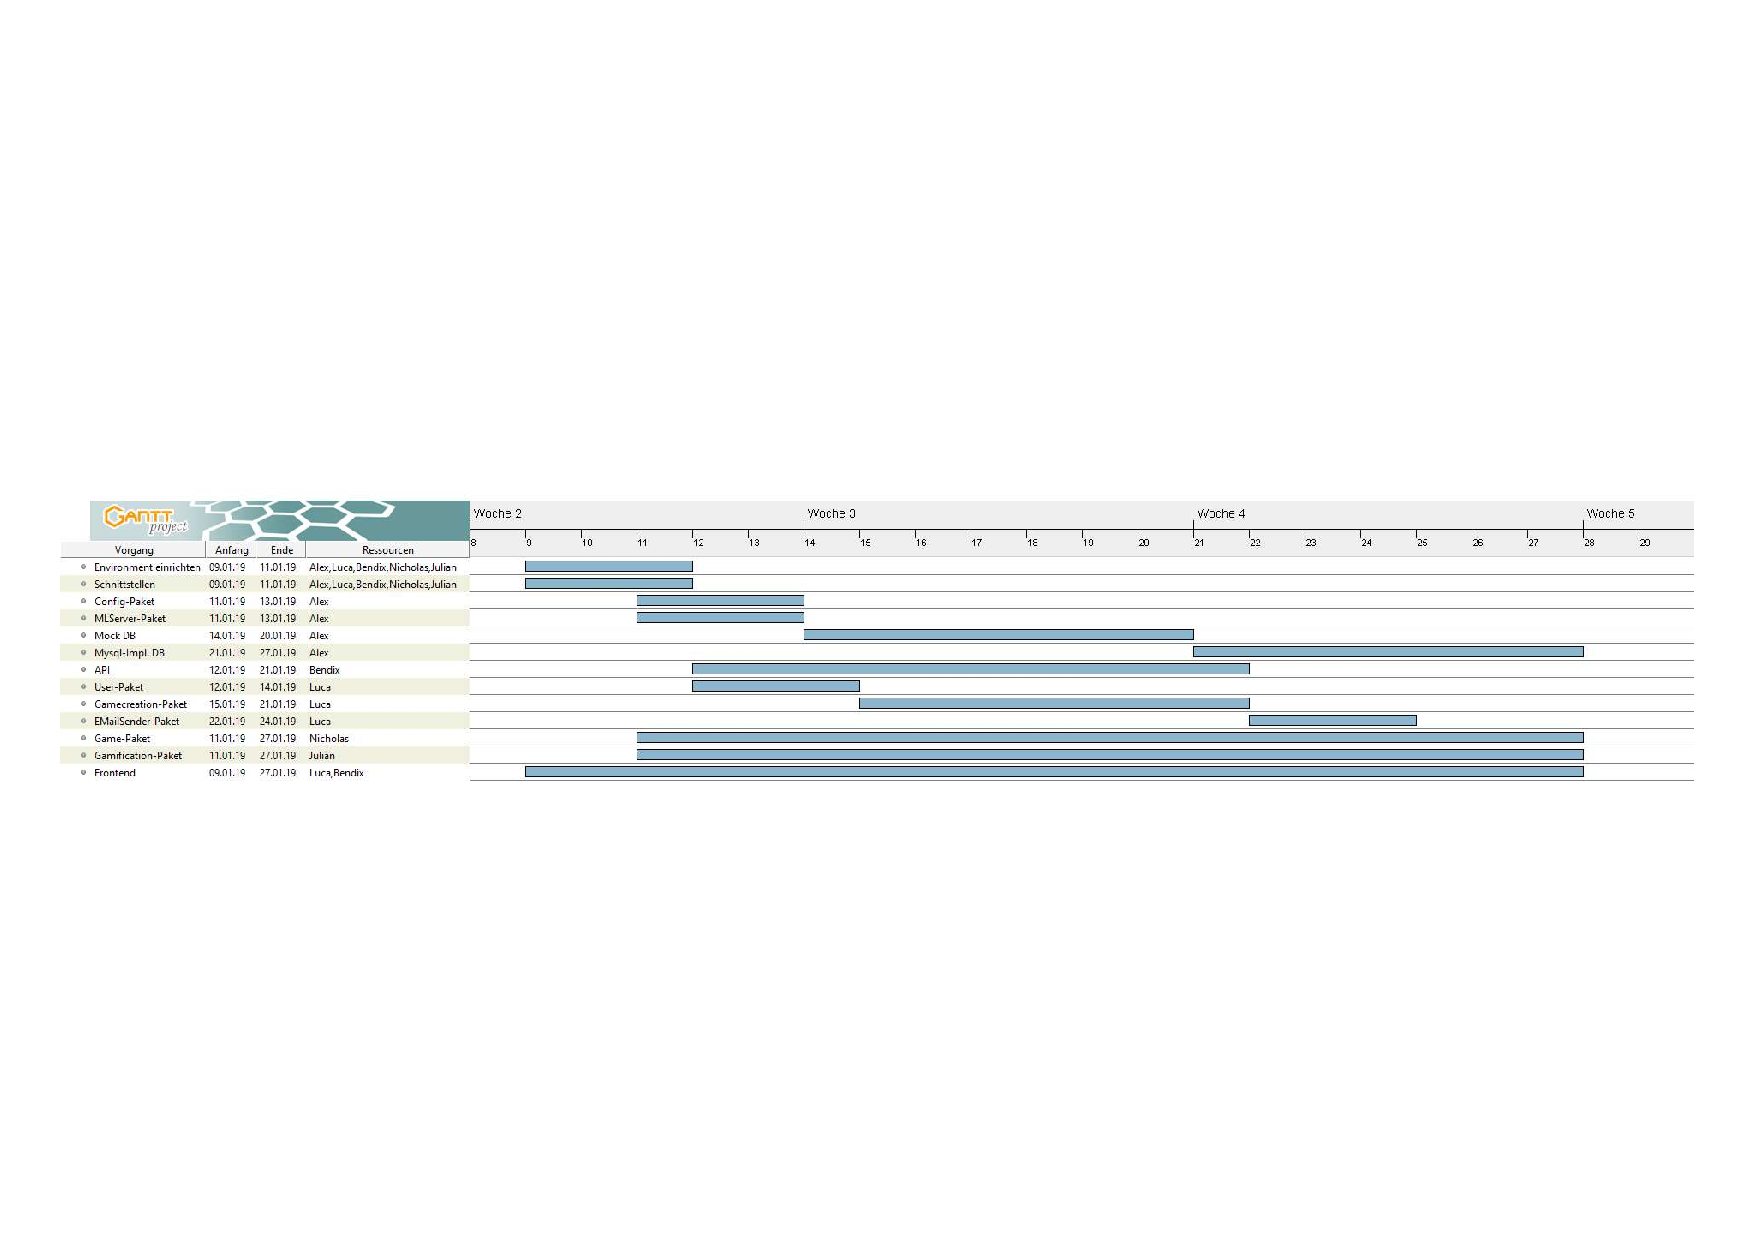
\includegraphics[width=\textwidth]{../img/gantt.pdf}
\end{figure}
\begin{itemize}
	\item Zeitplan weitestgehend eingehalten
	\item In letzter Woche hauptsächlich nur noch Arbeit am Front-End
	\item Problem: Funktioniert nicht mit aktueller MySQL-Version
\end{itemize}
\end{frame}

\section{Änderungen am Entwurf}
\begin{frame}{Database}
    \begin{itemize}
        \item Neue Oberklasse für alle Adapter
        \item Query-Klasse zur Bündelung von SQL-Statements
        \item PlayerStats-Adapter
        \item Auslagerung der Nutzerverwaltung in eigene Pakete
        \item FeatureSet Informationen verbleiben auf der Platte
    \end{itemize}
\end{frame}

\begin{frame}{Gamification}
  \begin{itemize}
     \item Größten Änderungen bei Achievements
     \item Enum AchievementType
     \item checkProgress erzeugt ein neues konkretes Achievement (mit Type und State)
     \item Kommunikation von PlayerStats mit Datenbank
  \end{itemize}
\end{frame}

\renewcommand{\arraystretch}{1.5}

\section{Statistiken}
\begin{frame}{Unit-Tests}
  \begin{center}
    \begin{tabular}{ | l | c | c | }
      \hline
      Paket & Testüberdeckung (\%) & Unit-Tests \\ \hline
      User & 60 & 16 \\
      Database & 62 & 44 \\
      Game & 74 & 45 \\
      Gamification & 96 & 34 \\
      Configuration & 76 & 10 \\
      \hline
    \end{tabular}
  \end{center}
\end{frame}

\begin{frame}{Lines of Code}
  \begin{itemize}
    \item Java: 7340 LOC, 2364 Kommentar-Zeilen \\
    \item JavaScript: 974 LOC \\
    \item JavaServerPages: 405 LOC \\
    \item XML: 322 LOC \\
    \item Properties: 282 Zeilen \\
    \item CSS: 59 LOC \\
    \item Alle Dateien: 13765 Zeilen \\
  \end{itemize}
\end{frame}
\section{Docker}
\begin{frame}{Docker}
\begin{itemize}
    \item Docker Compose
    \item Container
    \begin{itemize}
        \item MySql
        \item Tomcat
        \item ML-Server
    \end{itemize}
    \item Konnte MySql Version leicht anpassen
\end{itemize}
\end{frame}
\begin{frame}{GitHub - CS:Select}
  \begin{itemize}
    \item 570 Commits bis zur Abgabefrist \\
    \item 26 bearbeitete Issues in den letzten 2 Tagen vor Abgabefrist \\
  \end{itemize}
\end{frame}

\section{Entwicklungsmodell}
    \begin{frame}{Kommunikation im Team}
        \begin{itemize}
            \item WhatsApp
            \item TeamSpeak
            \item Github Issues
        \end{itemize}
    \end{frame}
    \begin{frame}{Verwendung von Git}
        \begin{itemize}
            \item Feature Branches
            \item Pull Requests auf Master
            \item Code Review vor Merge
            \item Kleinere Anpassungen direkt auf Master
        \end{itemize}
    \end{frame}

\end{document}
